\chapter{Resultados}\label{chap:resultados}

Este capítulo evalúa el sistema construido en el Capítulo~\ref{chap:metodologia} y analiza
su comportamiento desde la representación hasta la operación. El recorrido comienza en los
perfiles de aspecto que la canalización ABSA induce sobre los usuarios: primero se estudia
qué estructura poblacional exhiben (Sección~\ref{sec:res_perfiles}) y después se verifica
que sean coherentes con las visitas reales, tanto pasadas como futuras
(Sección~\ref{sec:res_coherencia}). Sobre esa base se comparan los tres modelos individuales
con pruebas de significancia (Sección~\ref{sec:res_modelos}), se examina cómo reparten sus
recomendaciones sobre el catálogo (Sección~\ref{sec:res_distribucion}) y cómo varía su
rendimiento con la cantidad de historial disponible (Sección~\ref{sec:res_segmentos}). La
Sección~\ref{sec:res_hibrido} presenta el barrido del peso de fusión y el frente de Pareto
que dan respuesta a la pregunta central del trabajo. El capítulo cierra con dos análisis de
operación: un estudio de caso que ilustra la capacidad explicativa del modelo de contenido
(Sección~\ref{sec:res_caso}) y una simulación que valida la incorporación de usuarios
nuevos mediante una encuesta inicial (Sección~\ref{sec:res_encuesta}). Salvo indicación en
contrario, todos los resultados se calculan sobre los 9,134 usuarios de la partición de
prueba, con $K=10$ como corte principal y con las matrices construidas según la variante D
del estudio de ablación.

% ============================================================
\section{Perfiles de aspecto de los usuarios}\label{sec:res_perfiles}

La matriz $\mathbf{X}$ asigna a cada usuario un vector de importancia sobre los ocho
aspectos. Antes de usar esos perfiles para recomendar conviene preguntarse qué estructura
poblacional inducen: ¿existen tipos de viajero reconocibles, o la representación solo
registra cuánto escribe cada quien? Para responderlo se aplicó agrupamiento $k$-medias
sobre dos representaciones complementarias del mismo perfil: las filas de $\mathbf{X}$
estandarizadas por aspecto, que conservan la magnitud absoluta de las importancias, y su
versión normalizada $w_{u,a} = X_{u,a} / \sum_{a'} X_{u,a'}$, que retiene únicamente la
orientación relativa del perfil y coincide con los pesos que emplea el modelo de contenido.
El número de grupos se seleccionó con el coeficiente de silueta
(Figura~\ref{fig:cluster_selection}).

\begin{figure}[ht]
	\centering
	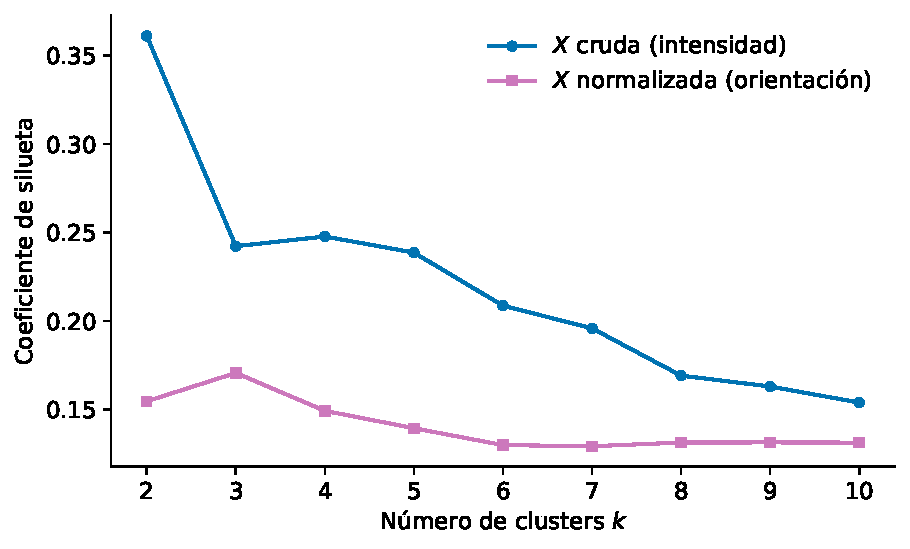
\includegraphics[width=0.62\textwidth]{figures/profiles_cluster_selection.pdf}
	\caption[Selección del número de clusters]{Coeficiente de silueta en función del número
		de clusters para las dos representaciones del perfil. La matriz cruda alcanza su
		máximo en $k=2$ y la normalizada en $k=3$.}
	\label{fig:cluster_selection}
\end{figure}

Las dos representaciones revelan dimensiones distintas y complementarias. Sobre la matriz
cruda la mejor partición es binaria y separa a los usuarios por la intensidad global de sus
menciones (Figura~\ref{fig:centroids_raw}): un grupo mayoritario con importancias bajas en
todos los aspectos y otro, cerca de un tercio de la población, con importancias
uniformemente altas. Los dos grupos comparten una composición similar de tipos de
establecimiento reseñados, de modo que esta dimensión no distingue gustos sino volumen de
escritura: la forma sigmoidal de la Ecuación~(\ref{eq:matrix_X}) traduce el número de
fragmentos en importancia, y el rasgo dominante de la población es cuánta evidencia textual
aporta cada usuario.

\begin{figure}[ht]
	\centering
	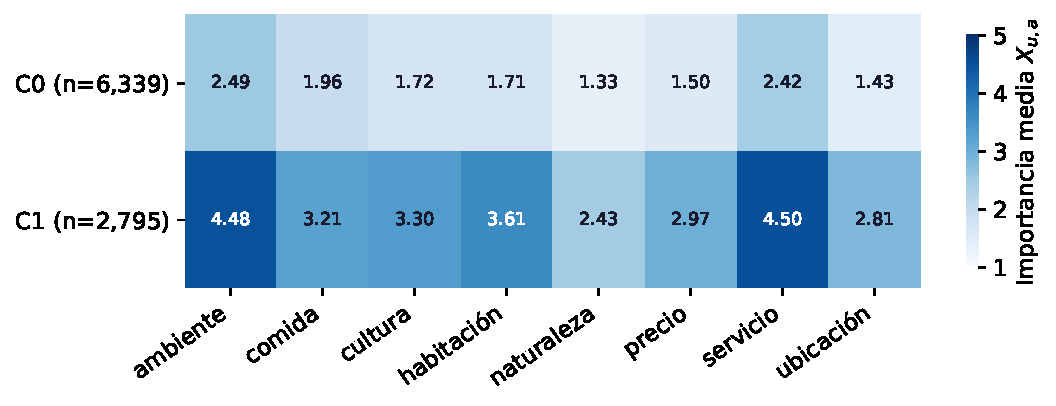
\includegraphics[width=0.78\textwidth]{figures/profiles_centroids.pdf}
	\caption[Centroides de los clusters de intensidad]{Centroides del agrupamiento sobre la
		matriz $\mathbf{X}$ cruda, en la escala original de importancia. La partición separa
		usuarios de baja y alta intensidad de mención, con el mismo orden relativo entre
		aspectos en ambos grupos.}
	\label{fig:centroids_raw}
\end{figure}

Al descontar la intensidad mediante la normalización aparece la estructura temática. La
mejor partición tiene tres grupos de tamaños comparables cuyos centroides se muestran en la
Figura~\ref{fig:centroids_norm}: un grupo orientado al hospedaje, que concentra su peso en
la habitación y la ubicación; un grupo orientado a los atractivos, con los mayores pesos
relativos en cultura y naturaleza; y un grupo gastronómico, cuyo aspecto dominante es la
comida. Esta lectura se valida externamente con la composición de las reseñas de cada
grupo: la mayoría de las reseñas del primer grupo proviene de hoteles, la del segundo de
atractivos turísticos y la del tercero de restaurantes. La proyección sobre las dos
primeras componentes principales (Figura~\ref{fig:pca_perfiles}) muestra los tres lóbulos
claramente diferenciados. En conjunto, el perfil ABSA codifica dos dimensiones
interpretables, la intensidad con que el usuario opina y la orientación temática de sus
opiniones, y la segunda coincide con el tipo de experiencia turística que el usuario
consume, lo que confirma que la canalización captura señal de preferencia y no solo ruido
de frecuencia.

\begin{figure}[ht]
	\centering
	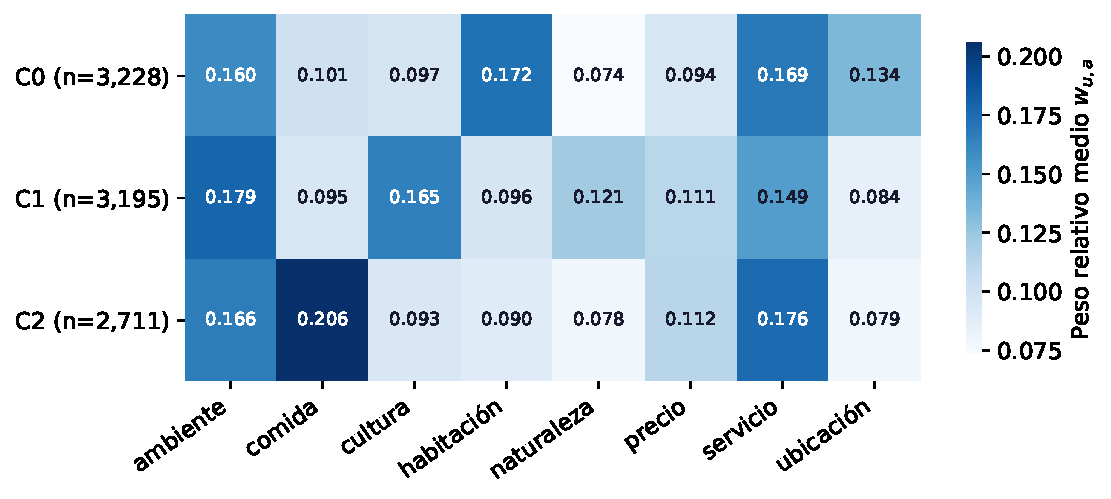
\includegraphics[width=0.78\textwidth]{figures/profiles_centroids_norm.pdf}
	\caption[Centroides de los clusters temáticos]{Centroides del agrupamiento sobre el
		perfil normalizado $w_{u,a}$. Cada grupo concentra su peso relativo en una familia de
		aspectos: hospedaje (C0), cultura y naturaleza (C1) y gastronomía (C2).}
	\label{fig:centroids_norm}
\end{figure}

\begin{figure}[ht]
	\centering
	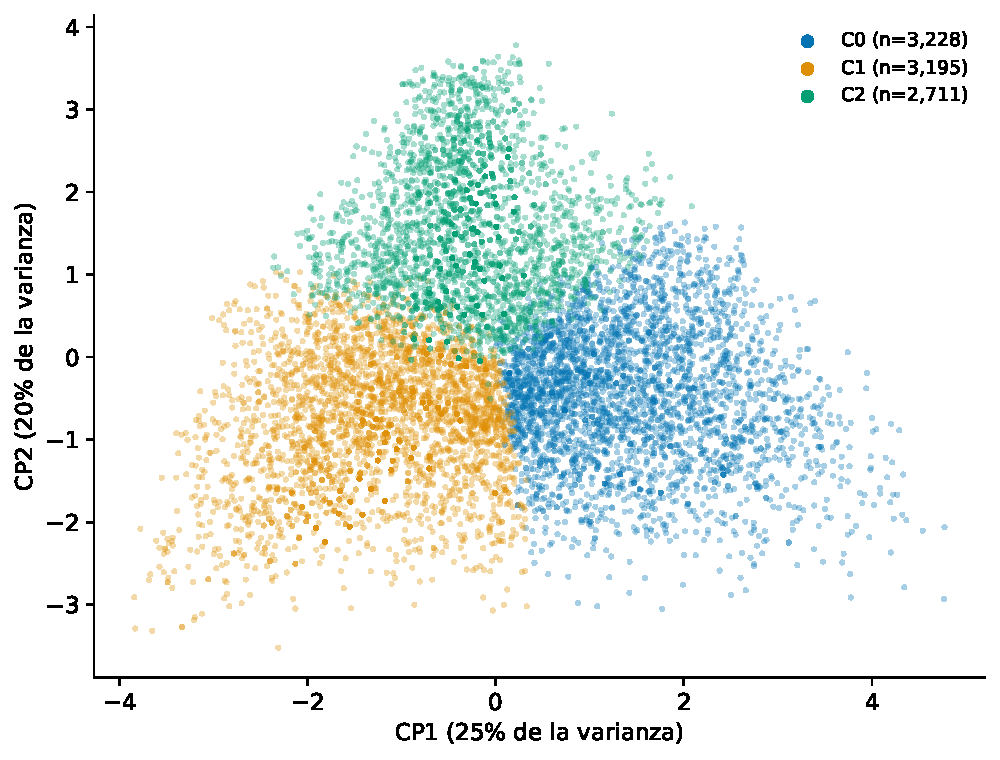
\includegraphics[width=0.62\textwidth]{figures/profiles_pca.pdf}
	\caption[Proyección PCA de los perfiles temáticos]{Proyección de los perfiles
		normalizados sobre las dos primeras componentes principales, coloreada por cluster
		temático. Los tres grupos ocupan regiones diferenciadas del espacio de aspectos.}
	\label{fig:pca_perfiles}
\end{figure}

% ============================================================
\section{Coherencia de los perfiles con las visitas}\label{sec:res_coherencia}

Que los perfiles exhiban estructura no garantiza que describan el comportamiento de viaje.
Esta sección cuantifica el ajuste entre el perfil de un usuario y los pueblos con los que
interactúa mediante la coherencia
\begin{equation}\label{eq:coherencia}
	\mathrm{coh}(u, S) = \mathrm{corr}\left( \mathbf{X}_u,\; \tfrac{1}{|S|}
	\textstyle\sum_{p \in S} \mathbf{Y}_p \right),
\end{equation}
la correlación de Pearson entre el vector de importancias del usuario y el perfil medio de
calidad de un conjunto $S$ de pueblos. Se evalúan cuatro conjuntos por usuario: su
historial de entrenamiento, sus visitas futuras (los pueblos de prueba), y las listas
top-10 de cada rama del híbrido. Una precaución metodológica resulta esencial: como todas
las filas de $\mathbf{Y}$ comparten un patrón común de aspectos populares, la coherencia
de un conjunto crece espuriamente con su tamaño, así que cada conjunto se contrasta contra
un nulo de conjuntos aleatorios del mismo tamaño y se reporta el exceso de coherencia
respecto de ese nulo. La Figura~\ref{fig:coherencia} resume las distribuciones y las
pruebas de Wilcoxon pareadas correspondientes.

\begin{figure}[ht]
	\centering
	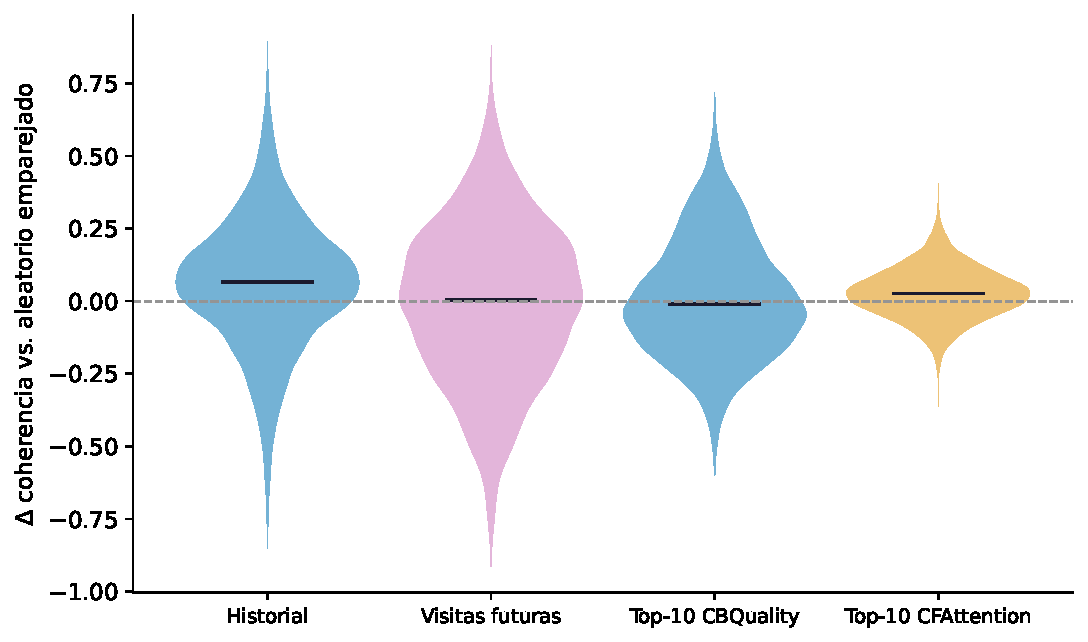
\includegraphics[width=0.75\textwidth]{figures/profiles_coherence.pdf}
	\caption[Coherencia perfil-visitas]{Distribución por usuario del exceso de coherencia
		de cada conjunto respecto de conjuntos aleatorios del mismo tamaño. La línea
		discontinua marca el nivel del azar; la barra negra, la mediana.}
	\label{fig:coherencia}
\end{figure}

El historial es significativamente más coherente que el azar (mediana del exceso
$+0.066$, $p < 10^{-4}$, $r = 0.28$), lo que confirma que el perfil resume las
preferencias expresadas en las visitas pasadas, en parte por construcción, pues
$\mathbf{X}$ se estima con los fragmentos escritos en esos mismos pueblos. El resultado
informativo aparece en los otros tres conjuntos. Las visitas futuras no son más coherentes
que el azar ($p = 0.59$): el destino siguiente de un usuario no se parece, en la forma de
su perfil de calidad, más de lo esperable a su patrón de importancias. Las listas del
modelo de contenido tampoco lo son ($p = 0.22$), a pesar de que CBQuality selecciona
maximizando el emparejamiento $\mathbf{X}_u \cdot \mathbf{Y}_p$; la explicación es que su
puntuación premia el nivel absoluto de calidad ponderado por la atención del usuario, no
el parecido de forma que mide la correlación, de modo que el modelo recomienda pueblos
sobresalientes en general y no pueblos con silueta de calidad similar al perfil. Las
listas de CFAttention, en cambio, sí presentan un exceso de coherencia pequeño pero muy
consistente ($r = 0.30$): al construir la vecindad en el espacio de aspectos, las
recomendaciones heredan la forma del perfil del usuario. Estos contrastes anticipan los
dos comportamientos de exposición que se documentan en la
Sección~\ref{sec:res_distribucion} y matizan la lectura del modelo de contenido: su
ventaja predictiva, que se cuantifica a continuación, proviene de identificar calidad
agregada relevante para el usuario más que de replicar la forma exacta de su perfil.

% ============================================================
\section{Evaluación de los modelos individuales}\label{sec:res_modelos}

La Tabla~\ref{tab:modelos} reúne el rendimiento de los tres modelos para
$K \in \{5, 10, 20\}$, evaluados sobre el mismo conjunto de usuarios de prueba. El patrón
es nítido y revela una complementariedad que motiva la fusión. CBQuality domina con
holgura en todas las métricas de relevancia y en todos los cortes: su NDCG@10 casi
triplica el de los dos modelos colaborativos, y otro tanto ocurre con la exhaustividad y
el acierto. Este resultado confirma que, bajo la fuerte dispersión del corpus, el
emparejamiento de perfiles de aspecto recupera preferencias que la escasa coincidencia de
calificaciones no permite estimar de forma fiable, en coherencia con las ventajas del
filtrado de contenido ante el problema del arranque en frío. El precio que paga CBQuality
es la cobertura: a $K=5$ expone menos de la mitad del catálogo, porque tiende a concentrar
sus recomendaciones en los pueblos de mayor calidad agregada. Los dos modelos
colaborativos exhiben el comportamiento opuesto, con cobertura prácticamente total desde
los cortes bajos pero con una relevancia muy inferior. Entre ellos, CFAttention y
CFClassic quedan próximos, lo que indica que medir la afinidad entre usuarios en el
espacio de aspectos no se traduce por sí sola en mejor ordenamiento, aunque sí aporta la
cobertura que a CBQuality le falta. Esta tensión entre relevancia y cobertura es la que el
modelo híbrido busca administrar.

\begin{table}[ht]
	\centering
	\caption{Rendimiento de los modelos individuales para distintos cortes $K$. P, R y NDCG
		denotan precisión, exhaustividad y \textit{ranking}; MRR el rango recíproco medio; ILD la
		diversidad intra-lista; y Cov la cobertura de catálogo.}
	\label{tab:modelos}
	\begin{tabular}{llrrrrrr}
		\toprule
		\textbf{Modelo} & \textbf{$K$} & \textbf{P@$K$} & \textbf{R@$K$} & \textbf{NDCG@$K$} & \textbf{MRR} & \textbf{ILD} & \textbf{Cov@$K$} \\
		\midrule
		CBQuality       & 5            & 0.102          & 0.446          & 0.312             & 0.275        & 0.001        & 0.479            \\
		                & 10           & 0.068          & 0.610          & 0.366             & 0.296        & 0.004        & 0.729            \\
		                & 20           & 0.045          & 0.811          & 0.418             & 0.310        & 0.008        & 0.958            \\
		\midrule
		CFClassic       & 5            & 0.033          & 0.150          & 0.091             & 0.076        & 0.008        & 1.000            \\
		                & 10           & 0.032          & 0.284          & 0.135             & 0.095        & 0.007        & 1.000            \\
		                & 20           & 0.029          & 0.527          & 0.197             & 0.112        & 0.007        & 1.000            \\
		\midrule
		CFAttention     & 5            & 0.030          & 0.133          & 0.081             & 0.068        & 0.008        & 0.979            \\
		                & 10           & 0.029          & 0.261          & 0.123             & 0.086        & 0.007        & 1.000            \\
		                & 20           & 0.029          & 0.525          & 0.190             & 0.104        & 0.007        & 1.000            \\
		\bottomrule
	\end{tabular}
\end{table}

Para descartar que estas diferencias se deban al azar se aplicó la prueba de rangos con
signo de Wilcoxon, pareada por usuario sobre el NDCG@10, con corrección de Holm por
comparaciones múltiples y el tamaño de efecto $r = |z| / \sqrt{n}$
(Tabla~\ref{tab:significancia}). Las tres comparaciones resultan significativas, pero los
tamaños de efecto cuentan dos historias distintas. La ventaja de CBQuality sobre ambos
modelos colaborativos es un efecto grande, mientras que la diferencia entre CFClassic y
CFAttention, aunque detectable gracias al tamaño muestral, es de magnitud casi nula. En la
práctica ambos colaborativos ordenan igual de bien, y la elección de CFAttention como rama
del híbrido se justifica por operar en el mismo espacio de aspectos que el resto del
sistema, no por una ganancia de relevancia.

\begin{table}[ht]
	\centering
	\caption{Pruebas de Wilcoxon pareadas por usuario sobre el NDCG@10 de los modelos
		individuales. $\Delta$ es la diferencia de medias; los p-valores incluyen la
		corrección de Holm; $r$ es el tamaño de efecto.}
	\label{tab:significancia}
	\begin{tabular}{llrcr}
		\toprule
		\textbf{Modelo A} & \textbf{Modelo B} & \textbf{$\Delta$ NDCG@10} & \textbf{$p$} & \textbf{$r$} \\
		\midrule
		CBQuality & CFClassic   & $+0.231$ & $<10^{-4}$ & 0.509 \\
		CBQuality & CFAttention & $+0.243$ & $<10^{-4}$ & 0.535 \\
		CFClassic & CFAttention & $+0.013$ & $<10^{-4}$ & 0.048 \\
		\bottomrule
	\end{tabular}
\end{table}

% ============================================================
\section{Distribución de las recomendaciones sobre el catálogo}\label{sec:res_distribucion}

Las métricas agregadas no revelan cómo se reparten las recomendaciones entre los 48
pueblos. Esta sección analiza la exposición de cada pueblo, definida como el número de
listas top-10 en que aparece, y muestra que detrás de la disyuntiva relevancia-cobertura
hay dos regímenes de distribución radicalmente distintos.

La Figura~\ref{fig:lorenz} presenta las curvas de Lorenz de la exposición. CBQuality
concentra sus recomendaciones de forma extrema, con un coeficiente de Gini de 0.75: la
mitad del catálogo apenas recibe exposición y trece pueblos no aparecen en ninguna lista.
Los dos modelos colaborativos reparten la exposición de manera mucho más equitativa, con
Gini cercano a 0.4 y sin pueblos excluidos, y el híbrido en su punto de operación se sitúa
entre ambos extremos. La Figura~\ref{fig:expo_pop} identifica el mecanismo: la exposición
de CBQuality crece de forma casi monótona con la popularidad del pueblo en entrenamiento
(correlación de Spearman de 0.90), con un comportamiento de umbral en el que solo los
destinos con gran volumen de reseñas alcanzan exposición masiva. Es la firma de un sesgo
de popularidad heredado: los pueblos con más reseñas acumulan más menciones positivas, la
señal volumen-ponderada de la Ecuación~(\ref{eq:matrix_Y}) los lleva a la parte alta de
$\mathbf{Y}$, y el modelo de contenido los recomienda a casi todos los usuarios. La
exposición de CFAttention, en cambio, es esencialmente independiente de la popularidad
(Spearman de 0.05): al predecir con desviaciones respecto de la media de cada vecino, las
vecindades locales del espacio de aspectos reparten las recomendaciones por todo el
catálogo.

\begin{figure}[ht]
	\centering
	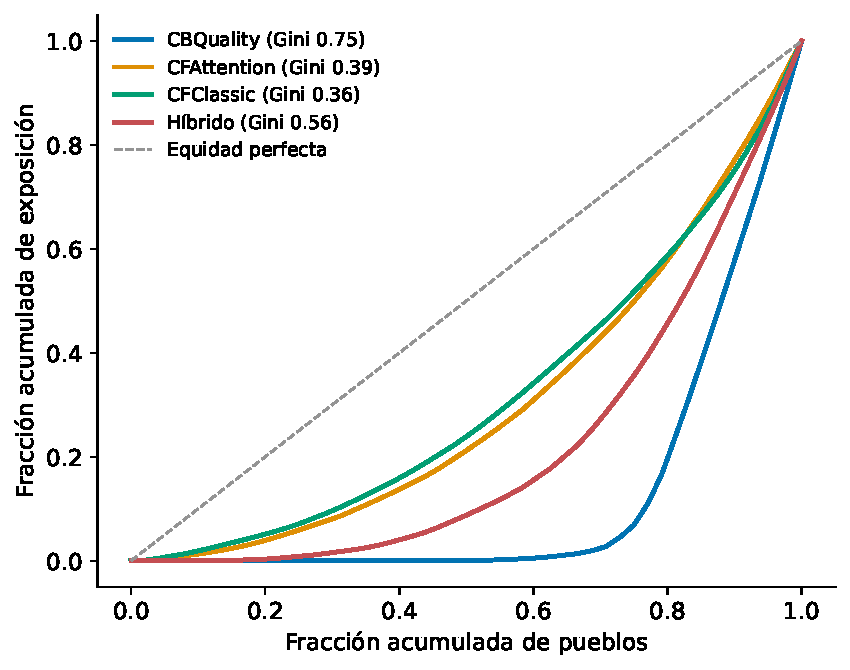
\includegraphics[width=0.6\textwidth]{figures/recs_lorenz.pdf}
	\caption[Curvas de Lorenz de la exposición]{Curvas de Lorenz de la exposición por
		pueblo en las listas top-10, con el coeficiente de Gini de cada modelo. El híbrido se
		evalúa en su punto de operación $\alpha^{\star}(\beta=0.5)$.}
	\label{fig:lorenz}
\end{figure}

\begin{figure}[ht]
	\centering
	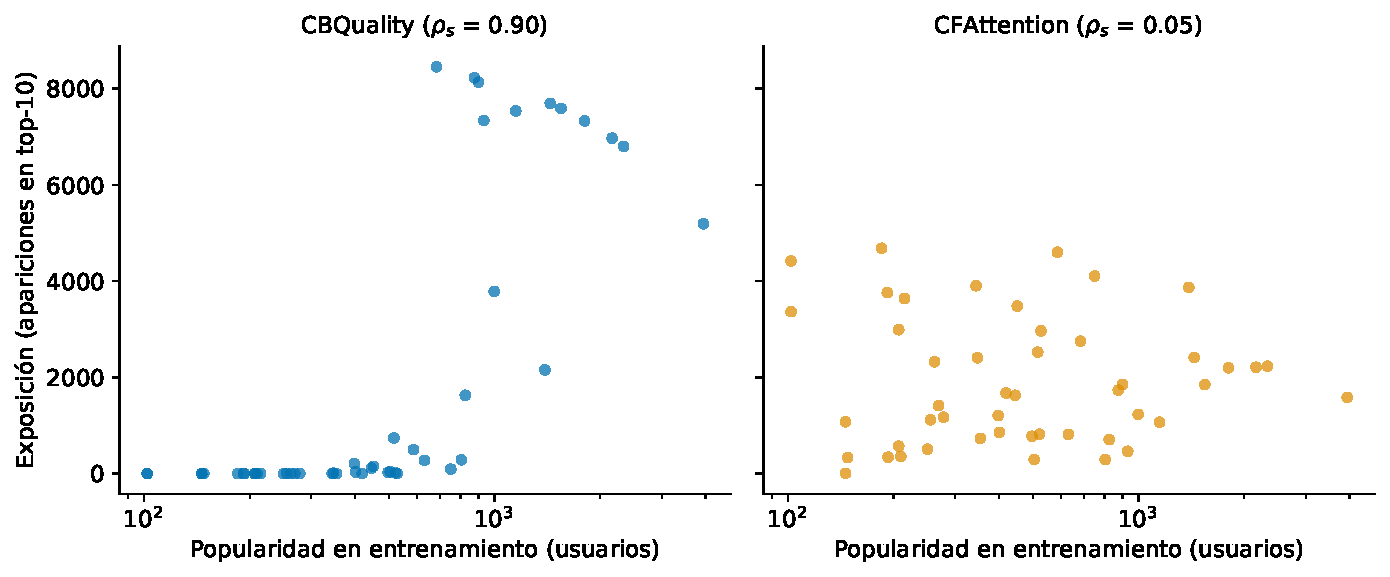
\includegraphics[width=0.9\textwidth]{figures/recs_exposure_popularity.pdf}
	\caption[Exposición frente a popularidad]{Exposición de cada pueblo en función de su
		popularidad en entrenamiento (escala logarítmica) para las dos ramas del híbrido, con
		la correlación de Spearman correspondiente. CBQuality exhibe un umbral de popularidad;
		CFAttention es prácticamente insensible a ella.}
	\label{fig:expo_pop}
\end{figure}

El mismo contraste se observa a nivel de usuario. Comparando el NDCG@10 de las dos ramas
usuario por usuario, CBQuality gana en el 56\% de los casos, CFAttention en el 13\% y el
31\% restante son empates, casi todos entre listas que no aciertan. La ventaja del modelo
de contenido es además transversal: se mantiene en los tres clusters temáticos de la
Sección~\ref{sec:res_perfiles} y en todos los niveles de historial, con su máximo entre
los usuarios de historial mínimo. Sin embargo, las listas de ambas ramas comparten en
promedio menos del 16\% de sus elementos, de modo que el colaborativo no es una versión
degradada del contenido sino una fuente de candidatos genuinamente distinta. Esa
complementariedad estructural es la que explota la fusión: la rama de contenido aporta el
acierto y la colaborativa el resto del catálogo, y por eso el híbrido puede ganar
cobertura sin renunciar del todo a la relevancia, como se cuantifica en la
Sección~\ref{sec:res_hibrido}.

% ============================================================
\section{Rendimiento por segmento de actividad}\label{sec:res_segmentos}

El esquema de partición deja historiales de entrenamiento de tamaño muy variable, desde un
solo pueblo hasta decenas. La Figura~\ref{fig:segmentos} desglosa el NDCG@10 y la
cobertura por segmento de historial, y muestra que la conclusión global es robusta: el
orden entre modelos se preserva en los cuatro segmentos, con CBQuality al frente en todos
ellos.

\begin{figure}[ht]
	\centering
	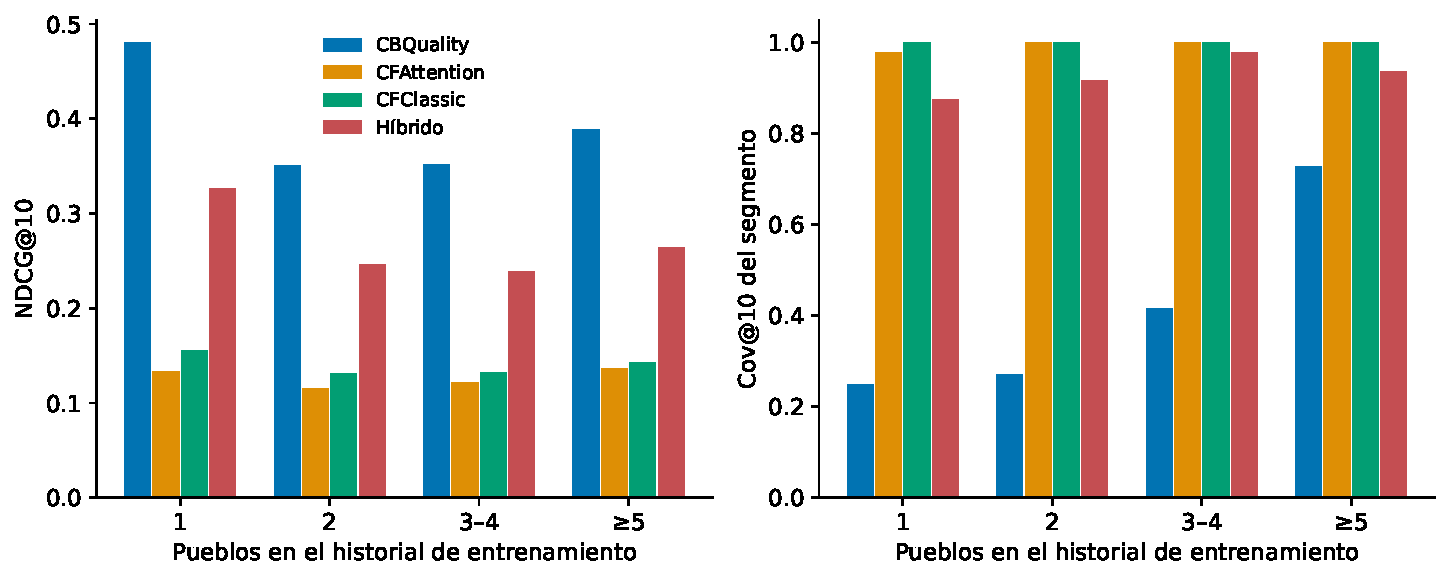
\includegraphics[width=0.95\textwidth]{figures/recs_segments.pdf}
	\caption[Rendimiento por segmento de actividad]{NDCG@10 (izquierda) y cobertura de
		catálogo dentro del segmento (derecha) según el número de pueblos en el historial de
		entrenamiento. El híbrido se evalúa en $\alpha^{\star}(\beta=0.5)$.}
	\label{fig:segmentos}
\end{figure}

Dos observaciones merecen destacarse. Primero, la relevancia de CBQuality no se degrada
con historiales cortos; de hecho alcanza su máximo en el segmento de un solo pueblo. El
perfil de aspectos se construye con los fragmentos de texto del usuario, no con la
coincidencia de sus calificaciones, así que unas pocas reseñas bastan para estimar una
representación útil. Este es precisamente el comportamiento deseable frente al arranque en
frío parcial, y anticipa la viabilidad de la encuesta de la
Sección~\ref{sec:res_encuesta}. Segundo, la cobertura de CBQuality sí depende fuertemente
del historial: en los segmentos cortos sus listas se concentran en una fracción pequeña
del catálogo y solo entre los usuarios más activos, cuyos pueblos populares ya fueron
visitados y quedan excluidos, el modelo se ve forzado a explorar destinos menos expuestos.
Los modelos colaborativos mantienen cobertura casi total en todos los segmentos. La
lectura conjunta refuerza el diagnóstico de la sección anterior: la limitación del modelo
de contenido no es de relevancia sino de exposición, y es una limitación estructural que
no desaparece con más historial de los usuarios típicos.

% ============================================================
\section{El híbrido y el compromiso relevancia--cobertura}\label{sec:res_hibrido}

La Figura~\ref{fig:alpha_sweep} traza el barrido del peso de fusión a $K=10$. El NDCG@10
desciende de forma monótona desde 0.366 en $\alpha=0$ hasta 0.118 en $\alpha=1$, con una
pendiente que se acentúa a partir de $\alpha \approx 0.6$. La cobertura recorre el camino
inverso: tras una breve meseta inicial, en la que incluso cede ligeramente respecto del
contenido puro, crece de manera sostenida hasta saturarse en la totalidad del catálogo
cerca de $\alpha = 0.96$. La relevancia proviene de CBQuality y la cobertura de
CFAttention, y no existe un valor de $\alpha$ que maximice ambas simultáneamente. Esta es
la manifestación empírica del compromiso multiobjetivo formalizado en la
Sección~\ref{sec:moo}.

\begin{figure}[ht]
	\centering
	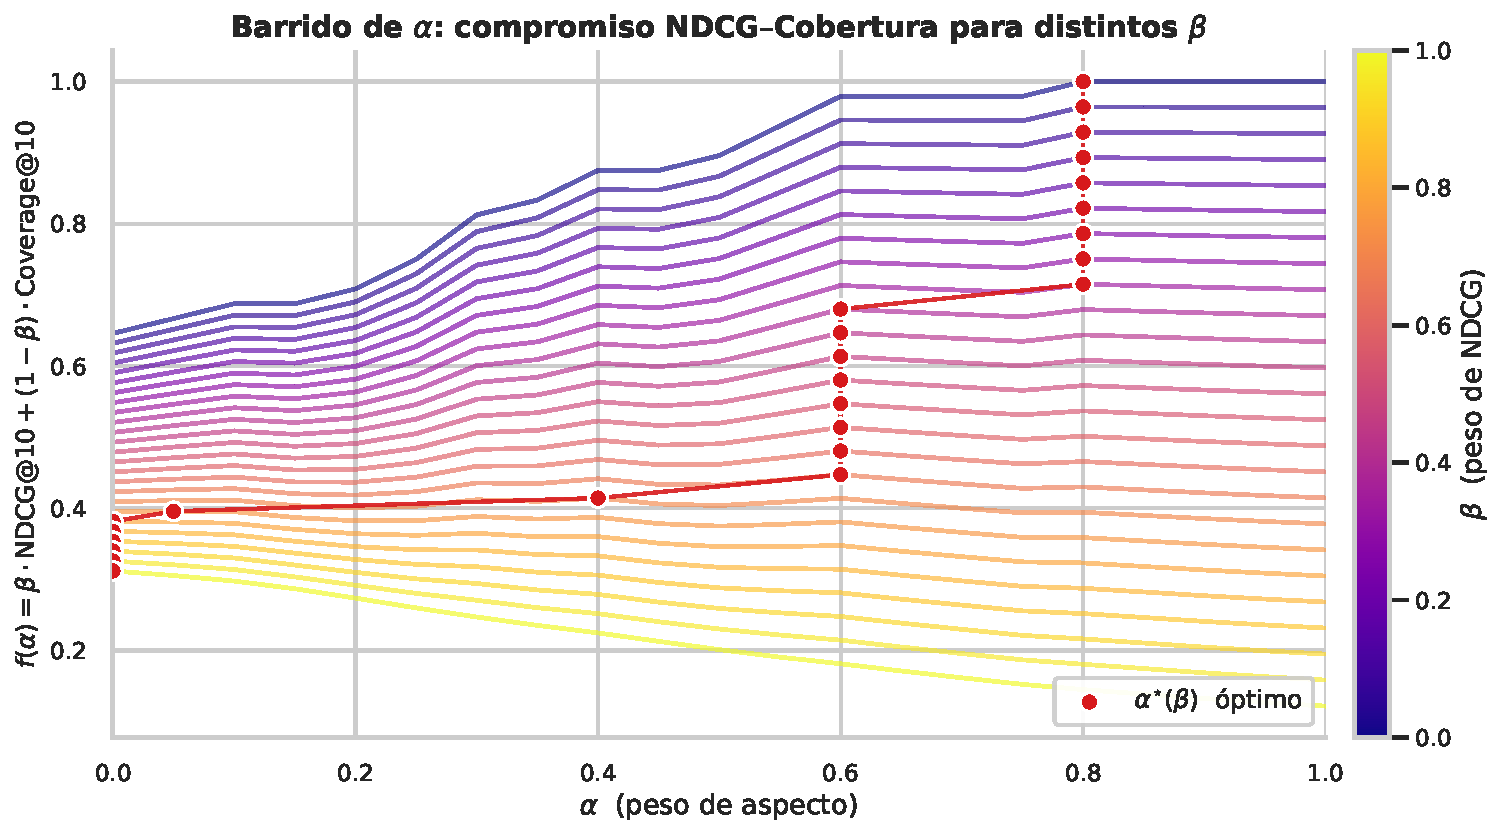
\includegraphics[width=0.72\textwidth]{figures/alpha_sweep.pdf}
	\caption[Barrido del peso de fusión]{Relevancia (NDCG@10) y cobertura (Cov@10) en función del
		peso de fusión $\alpha$. Al aumentar $\alpha$ la relevancia decrece y la cobertura crece
		hasta saturarse, lo que evidencia el conflicto entre ambos objetivos.}
	\label{fig:alpha_sweep}
\end{figure}

La Figura~\ref{fig:alpha_vs_beta} presenta el análisis de sensibilidad que resulta de
aplicar el criterio de selección de la Sección~\ref{sec:hibrido}, esto es, de escalarizar
ambos objetivos con el peso de preferencia $\beta$ y leer el óptimo
$\alpha^{\star}(\beta)$ directamente del barrido. La trayectoria del óptimo es una
escalera con tres regímenes. Cuando la preferencia se concentra en la cobertura, el óptimo
se instala en $\alpha^{\star} = 0.96$, el menor peso que ya alcanza cobertura total;
elevar $\alpha$ por encima solo sacrificaría relevancia sin ganar nada, así que esas
configuraciones quedan descartadas. En una amplia franja intermedia de preferencias el
óptimo se estabiliza en $\alpha^{\star} = 0.8$, y cuando la relevancia domina la decisión
el óptimo salta al modelo de contenido puro. Resulta notable la amplitud del régimen
central: para la mitad de las preferencias posibles la respuesta es la misma mezcla, un
híbrido cargado hacia la rama colaborativa que conserva cerca de dos tercios de la
relevancia del contenido puro con exposición casi completa del catálogo.

\begin{figure}[ht]
	\centering
	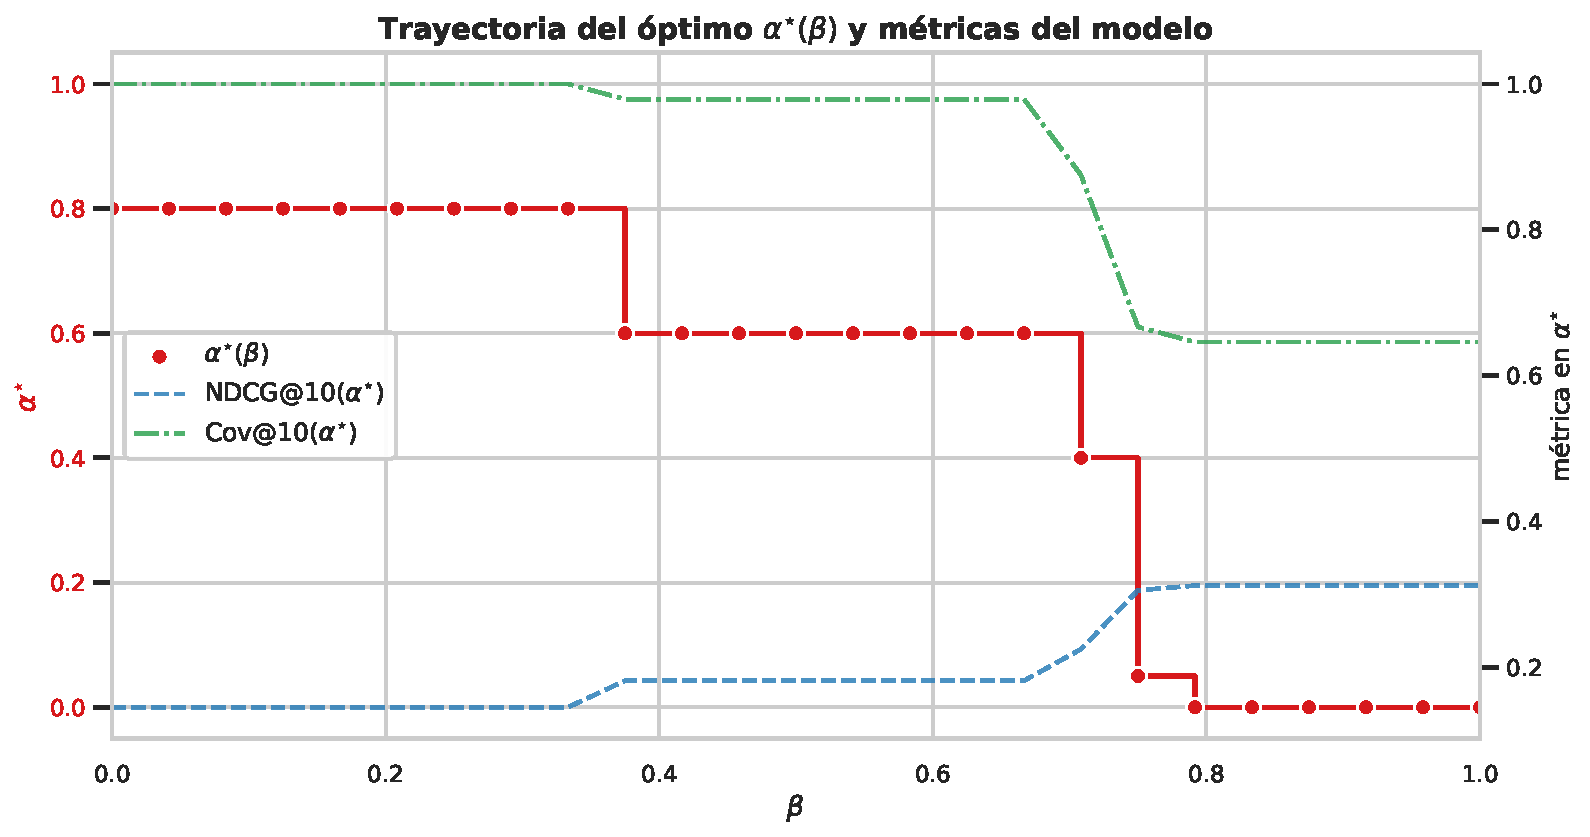
\includegraphics[width=0.75\textwidth]{figures/alphaVSbeta.pdf}
	\caption[Análisis de sensibilidad del óptimo]{Trayectoria del óptimo $\alpha^{\star}(\beta)$
		(escalera) y métricas alcanzadas en él. Al priorizar la relevancia ($\beta$ creciente) el
		óptimo se desplaza de un régimen colaborativo a uno de contenido puro, mientras la
		cobertura cede terreno y el NDCG@10 aumenta.}
	\label{fig:alpha_vs_beta}
\end{figure}

Finalmente, la Figura~\ref{fig:pareto_realized} representa el frente de Pareto realizado
del sistema en el plano cobertura-relevancia, el análogo empírico del frente teórico de la
Figura~\ref{fig:pareto_front}. Cada punto corresponde a un valor de $\alpha$; los puntos
no dominados forman la frontera eficiente sobre la que debe situarse cualquier elección
razonable de fusión. La frontera exhibe un codo pronunciado en $\alpha = 0.8$: hasta ese
punto la cobertura se compra barata, cediendo relevancia de forma gradual, mientras que
más allá el último tramo de cobertura exige un desplome de la relevancia. Ese codo
coincide con el régimen central de la escalera $\alpha^{\star}(\beta)$ y constituye el
punto de operación natural del sistema cuando no existe una preferencia fuerte hacia
ninguno de los dos objetivos. La mejora del híbrido en ese punto no es artefacto muestral:
frente a CFAttention, su ganancia de relevancia es significativa y de efecto grande
($r = 0.51$), y la pérdida frente a CBQuality, significativa pero de efecto medio
($r = 0.33$), es el costo cuantificado de exponer prácticamente todo el catálogo. La
elección final del peso de fusión deja así de ser una cuestión técnica para convertirse en
una decisión de diseño sobre cuánta relevancia se está dispuesto a ceder a cambio de
exponer una mayor parte del catálogo.

\begin{figure}[ht]
	\centering
	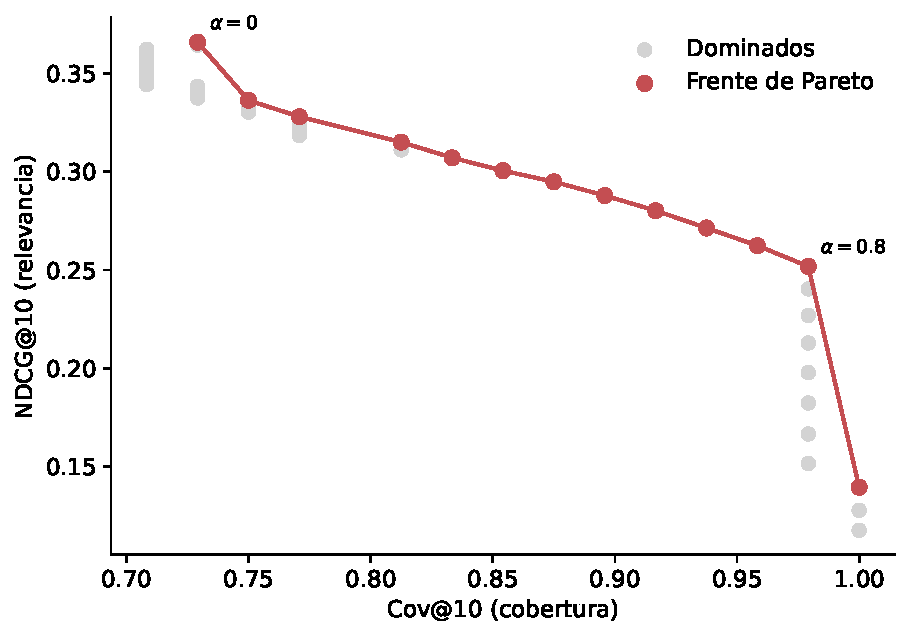
\includegraphics[width=0.68\textwidth]{figures/pareto_realized.pdf}
	\caption[Frente de Pareto realizado]{Frente de Pareto realizado del híbrido en el plano
		Cov@10--NDCG@10. Cada punto es un valor de $\alpha$; los puntos resaltados son no
		dominados y conforman la frontera eficiente, con un codo pronunciado en $\alpha=0.8$.}
	\label{fig:pareto_realized}
\end{figure}

% ============================================================
\section{Estudio de caso: recomendaciones explicables}\label{sec:res_caso}

Una ventaja del modelo de factores explícitos frente a los factores latentes es que sus
predicciones se descomponen en contribuciones interpretables. Como
$\hat{r}_{u,p} = \sum_a w_{u,a} Y_{p,a}$, la fracción $w_{u,a} Y_{p,a} / \hat{r}_{u,p}$
mide cuánto aporta cada aspecto a la recomendación y habilita explicaciones del tipo
``se recomienda este pueblo porque valoras la gastronomía y destaca en ella''. Para
ilustrarlo se seleccionó un usuario por cada cluster temático de la
Sección~\ref{sec:res_perfiles}, exigiendo historial mínimo de tres pueblos, acierto en su
lista top-10 y un perfil marcadamente orientado al aspecto firma de su grupo. La
Figura~\ref{fig:caso_perfiles} muestra sus perfiles y la Tabla~\ref{tab:caso} las
recomendaciones resultantes con sus contribuciones dominantes.

\begin{figure}[ht]
	\centering
	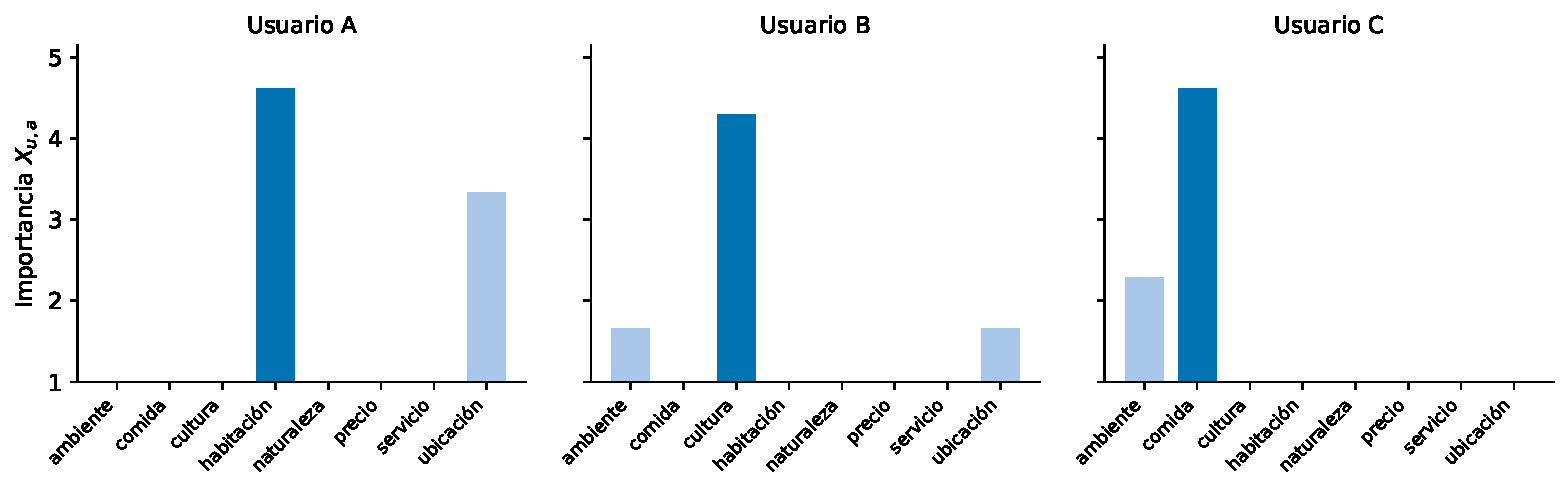
\includegraphics[width=0.95\textwidth]{figures/case_profiles.pdf}
	\caption[Perfiles de los usuarios del estudio de caso]{Perfiles de importancia
		$\mathbf{X}_u$ de los tres usuarios seleccionados, uno por cluster temático. El aspecto
		firma del cluster se resalta en tono oscuro; las barras en el mínimo de la escala
		corresponden a aspectos nunca mencionados.}
	\label{fig:caso_perfiles}
\end{figure}

\begin{table}[ht]
	\centering
	\caption{Top-3 de CBQuality para los tres usuarios del estudio de caso, con la fracción
		del puntaje aportada por los aspectos dominantes. La última columna indica si el pueblo
		apareció en las visitas futuras del usuario.}
	\label{tab:caso}
	\begin{tabular}{clllc}
		\toprule
		\textbf{Usuario} & \textbf{\#} & \textbf{Pueblo} & \textbf{Contribuciones principales} & \textbf{Acierto} \\
		\midrule
		A (hospedaje)   & 1 & Isla Mujeres               & habitación 33\%, ubicación 24\% &            \\
		                & 2 & San Cristóbal de las Casas & habitación 33\%, ubicación 24\% &            \\
		                & 3 & Bacalar                    & habitación 33\%, ubicación 24\% &            \\
		\midrule
		B (cultura)     & 1 & Tulum                      & cultura 34\%, ambiente 13\%     &            \\
		                & 2 & Isla Mujeres               & cultura 34\%, ambiente 13\%     &            \\
		                & 3 & Palenque                   & cultura 34\%, ambiente 13\%     &            \\
		\midrule
		C (gastronomía) & 1 & Tulum                      & comida 36\%, ambiente 18\%      &            \\
		                & 2 & Isla Mujeres               & comida 36\%, ambiente 18\%      &            \\
		                & 3 & Bacalar                    & comida 36\%, ambiente 18\%      & \checkmark \\
		\bottomrule
	\end{tabular}
\end{table}

Los tres casos ilustran el mecanismo explicativo y, al mismo tiempo, sus límites. El
usuario A, orientado al hospedaje, recibe recomendaciones justificadas por la habitación y
la ubicación; el usuario B, de perfil cultural, recibe destinos arqueológicos y coloniales
explicados por la cultura; y para el usuario C la gastronomía domina cada puntaje, con un
acierto directo en sus visitas futuras. La explicación es fiel al modelo, no una
racionalización a posteriori, porque reproduce exactamente la aritmética de la
predicción. Ahora bien, los conjuntos recomendados se parecen mucho entre usuarios: los
mismos destinos de alta calidad agregada aparecen en las tres listas y lo que cambia es la
justificación y el ordenamiento fino. Es la manifestación individual de la concentración
de exposición de la Sección~\ref{sec:res_distribucion}, y delimita el papel real de la
personalización en el modelo de contenido: personaliza la explicación y el orden más que
el conjunto de candidatos.

% ============================================================
\section{Usuarios nuevos: perfil por encuesta}\label{sec:res_encuesta}

El sistema descansa en perfiles extraídos de reseñas, de modo que un usuario recién
llegado, sin texto del cual extraer aspectos, plantea el caso extremo del arranque en
frío. La arquitectura ofrece una solución natural: como las entradas de $\mathbf{X}$ viven
en la escala $[1, 5]$, una encuesta de incorporación con ocho preguntas del tipo ``del 1
al 5, ¿cuánto te importa cada aspecto?'' produce directamente un perfil sintético
$\mathbf{X}_u$ en la representación que ambas ramas consumen. CBQuality puede puntuar de
inmediato el catálogo completo con ese perfil, y CFAttention puede construir la vecindad
del nuevo usuario en el espacio de aspectos y predecir con las calificaciones de sus
vecinos, sin requerir historial propio.

La pregunta empírica es cuánta calidad de recomendación se pierde al sustituir el perfil
continuo minado por ABSA por las respuestas discretas de una encuesta. Para estimarlo se
simuló la encuesta sobre los usuarios de prueba cuantizando su perfil real a los niveles
que el cuestionario capturaría, con dos granularidades: cinco niveles (redondeo al entero
más cercano) y tres niveles. La Tabla~\ref{tab:encuesta} y la Figura~\ref{fig:cold_start}
comparan el sistema completo bajo las tres fuentes de perfil.

\begin{table}[ht]
	\centering
	\caption{Simulación del perfil por encuesta: métricas a $K=10$ al sustituir el perfil
		continuo por su versión cuantizada. El híbrido se evalúa en
		$\alpha^{\star}(\beta=0.5)$.}
	\label{tab:encuesta}
	\begin{tabular}{lcccccc}
		\toprule
		& \multicolumn{2}{c}{\textbf{CBQuality}} & \multicolumn{2}{c}{\textbf{CFAttention}} & \multicolumn{2}{c}{\textbf{Híbrido}} \\
		\cmidrule(lr){2-3} \cmidrule(lr){4-5} \cmidrule(lr){6-7}
		\textbf{Perfil} & NDCG & Cov & NDCG & Cov & NDCG & Cov \\
		\midrule
		Continuo (ABSA)    & 0.366 & 0.729 & 0.122 & 1.000 & 0.252 & 0.979 \\
		Encuesta 5 niveles & 0.366 & 0.729 & 0.122 & 1.000 & 0.249 & 0.979 \\
		Encuesta 3 niveles & 0.365 & 0.729 & 0.122 & 1.000 & 0.247 & 0.958 \\
		\bottomrule
	\end{tabular}
\end{table}

\begin{figure}[ht]
	\centering
	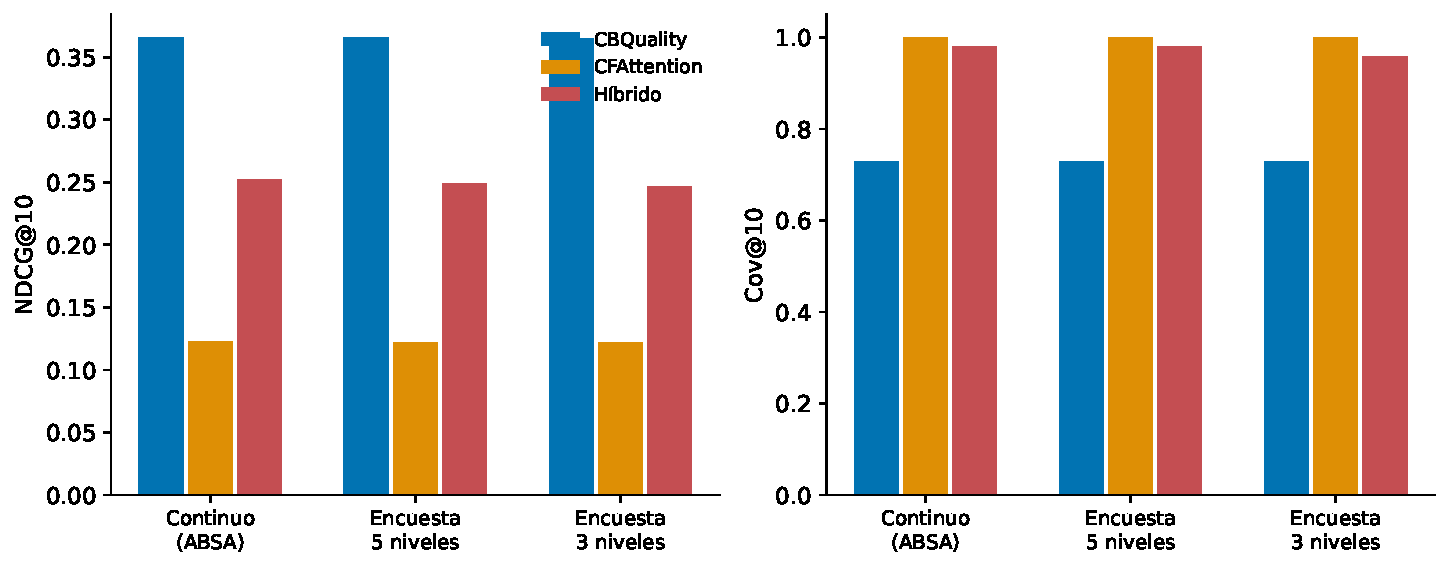
\includegraphics[width=0.9\textwidth]{figures/cold_start.pdf}
	\caption[Simulación del perfil por encuesta]{NDCG@10 (izquierda) y Cov@10 (derecha) del
		sistema según la fuente del perfil de usuario: continuo minado por ABSA, encuesta de
		cinco niveles y encuesta de tres niveles.}
	\label{fig:cold_start}
\end{figure}

La degradación es prácticamente nula. Con la encuesta de cinco niveles las listas top-10
del modelo de contenido conservan el 99\% de sus elementos y la correlación de rangos por
usuario entre ambos puntajes es casi perfecta; incluso la versión de tres niveles retiene
el 98\% de las listas y todas las métricas dentro del medio punto porcentual. La
información del perfil que el sistema realmente explota reside en niveles gruesos de
importancia, no en la precisión decimal de la frecuencia de menciones, así que ocho
respuestas bastan para situar a un usuario nuevo en igualdad de condiciones con uno cuyo
historial completo fue minado por la canalización. La simulación tiene una limitación que
conviene explicitar: asume que el usuario declararía en la encuesta lo mismo que sus
reseñas revelan, cuando la literatura sobre preferencias declaradas documenta sesgos de
auto-reporte. Validar esa correspondencia con usuarios reales queda como trabajo futuro;
lo que este experimento establece es que la representación no es el cuello de botella, y
que la vía de incorporación por encuesta es viable sin modificar ninguna pieza del
sistema.
